\hypertarget{stress_8cpp}{\section{stress.\-cpp \-File \-Reference}
\label{d4/d58/stress_8cpp}\index{stress.\-cpp@{stress.\-cpp}}
}


\-Definition of the member functions if the \hyperlink{classStress}{\-Stress} class.  


{\ttfamily \#include \char`\"{}stress.\-h\char`\"{}}\*
\-Include dependency graph for stress.\-cpp\-:\nopagebreak
\begin{figure}[H]
\begin{center}
\leavevmode
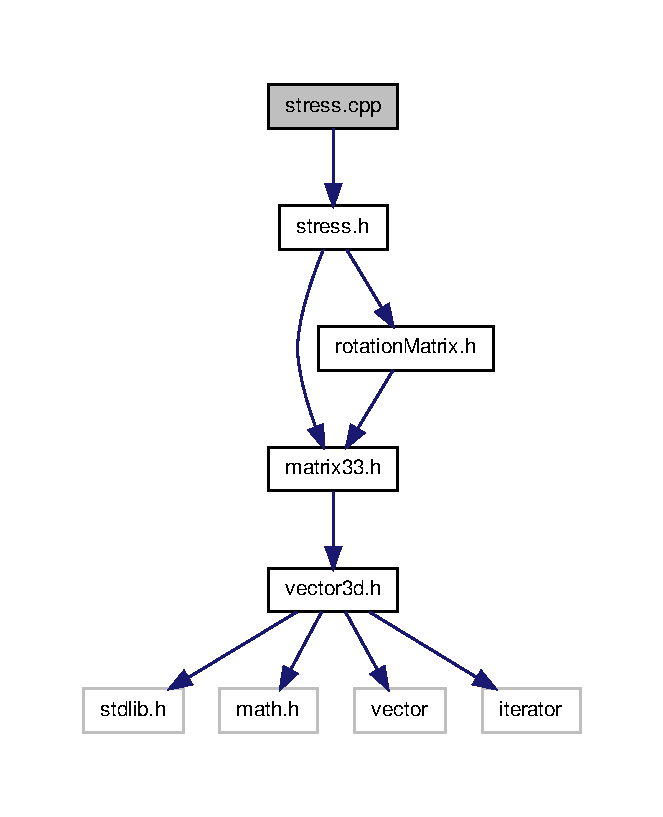
\includegraphics[width=142pt]{d0/d28/stress_8cpp__incl}
\end{center}
\end{figure}


\subsection{\-Detailed \-Description}
\-Definition of the member functions if the \hyperlink{classStress}{\-Stress} class. \begin{DoxyAuthor}{\-Author}
\-Adhish \-Majumdar 
\end{DoxyAuthor}
\begin{DoxyVersion}{\-Version}
0.\-0 
\end{DoxyVersion}
\begin{DoxyDate}{\-Date}
22/04/2013
\end{DoxyDate}
\-This file defines the member functions of the \hyperlink{classStress}{\-Stress} class for the stress tensor. 

\-Definition in file \hyperlink{stress_8cpp_source}{stress.\-cpp}.

